\chapter{Simulation Study} \label{chap:simulation}

\section{Simulated data}

\section{Models}
%
\begin{figure}[h]
	\centering
	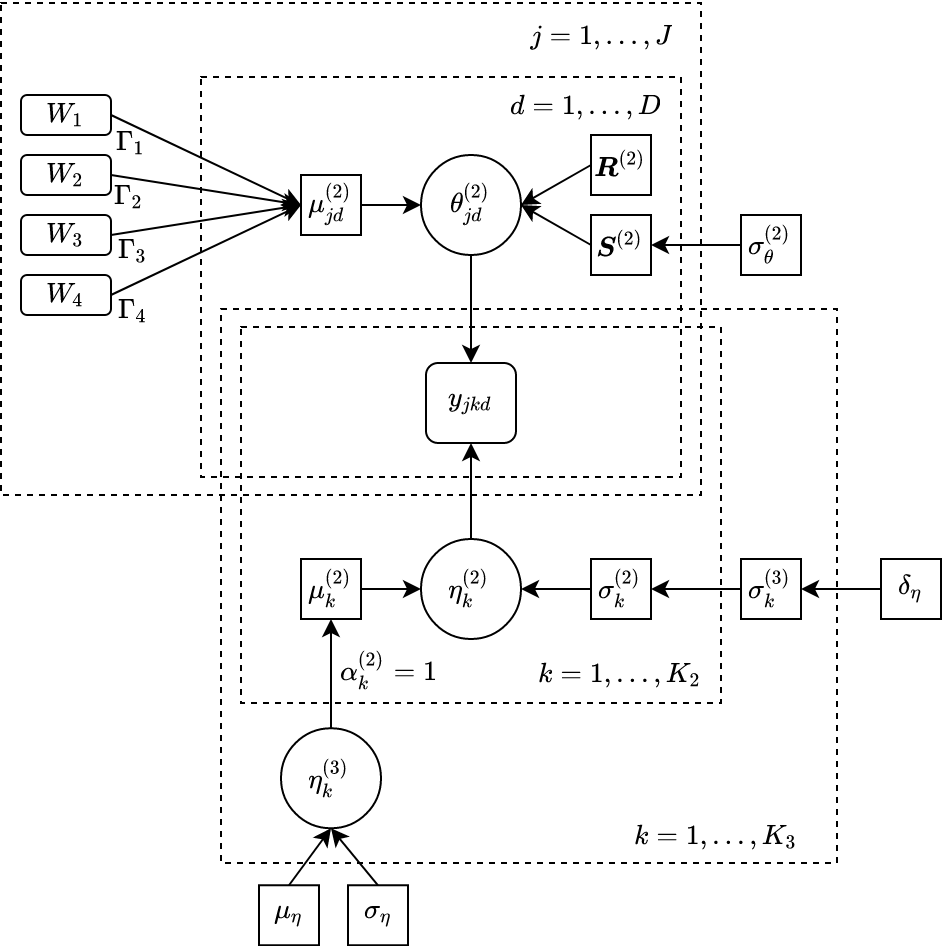
\includegraphics[width=0.7\linewidth]{4_FOLV_dag}
	%
	\caption[Directed Acyclig Graph (DAG). First Order Latent Variables model (FOLV).]%
	{Directed Acyclig Graph (DAG). First Order Latent Variables model (FOLV). Circles represent latent variables. Squares represent parameters for priors. Large Squares represent nesting in specific units.}
	\label{fig:FOLV_model}
\end{figure}

%
\begin{figure}[h]
	\centering
	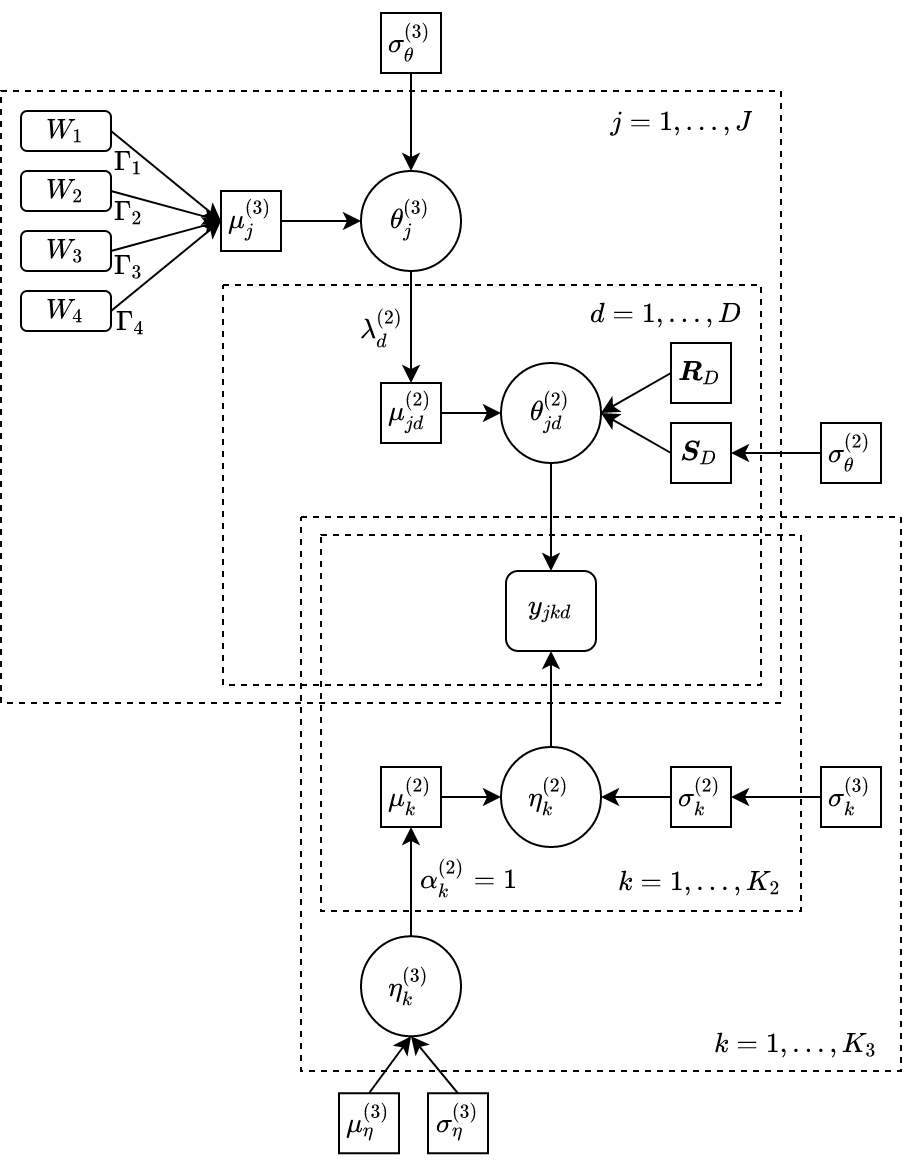
\includegraphics[width=0.7\linewidth]{4_SOLV_dag}
	%
	\caption[Directed Acyclig Graph (DAG). Second Order Latent Variables model (SOLV).]%
	{Directed Acyclig Graph (DAG). Second Order Latent Variables model (SOLV). Circles represent latent variables. Squares represent parameters for priors. Large Squares represent nesting in specific units.}
	\label{fig:SOLV_model}
\end{figure}


\section{Results}


